\documentclass[11pt, a4paper]{article}

\usepackage[english]{babel}
\usepackage{sleek}
\usepackage{common}

\title{Introduction to Artificial Intelligence (INFO8006)}
\subtitle{Exercises 7 -- Reinforcement learning}
\date{\today}

\begin{document}

\maketitle

\section*{Learning outcomes}

At the end of this session you should be able to
\begin{itemize}[noitemsep]
    \item differentiate passive and active RL;
    \item define and apply direct utility estimation and temporal-difference learning;
    \item define and apply $Q$-learning.
\end{itemize}

\section{Passive RL}

\begin{figure}[h]
    \centering
    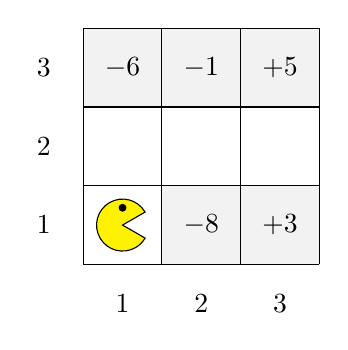
\begin{tikzpicture}
        \draw[step=1cm, black, thin] (0,0) grid (3,3);
        \fill[black, fill opacity=0.05] (1,0) rectangle (3,1);
        \fill[black, fill opacity=0.05] (0,2) rectangle (3,3);

        \draw[black, thin, fill=yellow] (0.5, 0.5) -- ++(30:0.33) arc (30:330:0.33) -- cycle;
        \fill[black] (0.5, 0.72) circle (0.05);

        \draw (0.5, -0.5) node {1};
        \draw (1.5, -0.5) node {2};
        \draw (2.5, -0.5) node {3};
        \draw (-0.5, 0.5) node {1};
        \draw (-0.5, 1.5) node {2};
        \draw (-0.5, 2.5) node {3};

        \draw (1.5, 0.5) node {$-8$};
        \draw (2.5, 0.5) node {$+3$};
        \draw (0.5, 2.5) node {$-6$};
        \draw (1.5, 2.5) node {$-1$};
        \draw (2.5, 2.5) node {$+5$};
    \end{tikzpicture}
    \vspace{-1ex}
\end{figure}

Consider the grid-world given above and an agent who is trying to learn the optimal policy. The agent starts from the bottom-left corner and can take the actions \texttt{north} ($N$), \texttt{south} ($S$), \texttt{west} ($W$) and \texttt{east} ($E$). Rewards are only awarded for reaching the terminal (shaded) states. You observe the following trials, whose trajectories are sequences of tuples $(s^i_t, r^i_t, a^i_t, s^i_{t+1})$.

\begin{table}[h]
    \centering
    \resizebox{0.95\textwidth}{!}{%
    \begin{tabular}{c|ccccc}
        \toprule
         $t$ & Trial 1 & Trial 2 & Trial 3 & Trial 4 & Trial 5 \\
         \midrule
         0 & $(1, 1), 0, N, (1, 2)$ & $(1, 1), 0, N, (1, 2)$ & $(1, 1), 0, N, (1, 2)$ & $(1, 1), 0, N, (1, 2)$ & $(1, 1), 0, N, (1, 2)$ \\
         1 & $(1, 2), 0, E, (2, 2)$ & $(1, 2), 0, E, (2, 2)$ & $(1, 2), 0, E, (2, 2)$ & $(1, 2), 0, E, (2, 2)$ & $(1, 2), 0, E, (2, 2)$ \\
         2 & $(2, 2), 0, N, (2, 3)$ & $(2, 2), 0, E, (3, 2)$ & $(2, 2), 0, S, (2, 1)$ & $(2, 2), 0, E, (3, 2)$ & $(2, 2), 0, E, (3, 2)$ \\
         3 & $(2, 3), -1, \varnothing, \varnothing$ & $(3, 2), 0, N, (3, 3)$ & $(2, 1), -8, \varnothing, \varnothing$ & $(3, 2), 0, W, (2, 2)$ & $(3, 2), 0, S, (3, 1)$ \\
         4 & & $(3, 3), +5, \varnothing, \varnothing$ & & $(2, 2), 0, N, (2, 3)$ & $(3, 1), +3, \varnothing, \varnothing$ \\
         5 & & & & $(2, 3), -1, \varnothing, \varnothing$ & \\
         \bottomrule
    \end{tabular}}
\end{table}

Assuming a discount factor $\gamma = 1$,

\begin{enumerate}
    \item Perform direct utility estimation of the expected utilities $V^\pi(s)$, given the four first trials.

    \begin{solution}
        In this setting, the transition model $P(s' | s, a)$ and the reward function $R(s)$ are unknown. We wish to learn the expected utility $V^\pi$ of the policy $\pi$ without modeling the environment, \ie{} without building approximates $\hat{P}(s' | s, a)$ and $\hat{R}(s)$. The principle of direct utility estimation is to approximate $V^\pi(s)$ by the average utility $\hat{V}(s)$ of the state $s$ within all trial trajectories, \ie{}
        \begin{equation*}
            \hat{V}(s) = \frac{1}{N(s)} \sum_{(i, j) \in I(s)} \sum_{t = 0}^{\infty} \gamma^t r^i_{j + t} \approx V^\pi(s) = \left. \E \sbk*{\sum_{t = 0}^{\infty} \gamma^t R(s_t)} \right|_{s_0 = s}
        \end{equation*}
        where $I(s) = \cbk{(i, j): s^i_j = s}$ indexes the occurrences of $s$ and $N(s) = \abs{I(s)}$ is the number of occurrences of $s$. For examples, in our case and excluding the fifth trial,
        \begin{align*}
            I((1, 1)) & = \cbk{(1, 0), (2, 0), (3, 0), (4, 0)} \\
            \hat{V}((1, 1)) & \approx \frac{1}{4} \rbk*{- 1 \, \gamma^3 + 5 \, \gamma^4 - 8 \, \gamma^3 - 1 \, \gamma^5} = \frac{-5}{4} \\
            I((2, 2)) & = \cbk{(1, 2), (2, 2), (3, 2), (4, 2), (4, 4)} \\
            \hat{V}((2, 2)) & \approx \frac{1}{5} \rbk*{- 1 \, \gamma^1 + 5 \, \gamma^2 - 8 \, \gamma^1 - 1 \, \gamma^3 - 1 \, \gamma^1} = \frac{-6}{5} \\
            I((2, 3)) & = \cbk{(1, 3), (4, 5)} \\
            \hat{V}((2, 3)) & \approx \frac{1}{2} \rbk*{- 1 \, \gamma^0 - 1 \, \gamma^0} = -1 .
        \end{align*}
        Importantly, since the agent hasn't reached the states $(1, 3)$ and $(3, 3)$ yet, it is not possible to estimate their expected utility. Instead, we assume a default value of $0$.

        \begin{figure}[h]
            \centering
            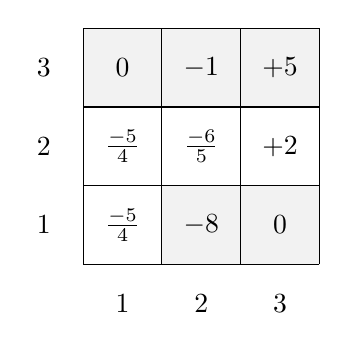
\begin{tikzpicture}
                \draw[step=1cm, black, thin] (0,0) grid (3,3);
                \fill[black, fill opacity=0.05] (1,0) rectangle (3,1);
                \fill[black, fill opacity=0.05] (0,2) rectangle (3,3);

                \draw (0.5, -0.5) node {1};
                \draw (1.5, -0.5) node {2};
                \draw (2.5, -0.5) node {3};
                \draw (-0.5, 0.5) node {1};
                \draw (-0.5, 1.5) node {2};
                \draw (-0.5, 2.5) node {3};

                \draw (0.5, 0.5) node {$\frac{-5}{4}$};
                \draw (1.5, 0.5) node {$-8$};
                \draw (2.5, 0.5) node {0};
                \draw (0.5, 1.5) node {$\frac{-5}{4}$};
                \draw (1.5, 1.5) node {$\frac{-6}{5}$};
                \draw (2.5, 1.5) node {$+2$};
                \draw (0.5, 2.5) node {0};
                \draw (1.5, 2.5) node {$-1$};
                \draw (2.5, 2.5) node {$+5$};
            \end{tikzpicture}
        \end{figure}
    \end{solution}

    \item Update the estimated expected utilities with respect to the fifth trial using temporal-difference learning. Assume a learning rate $\alpha = 0.5$.

    \begin{solution}
        Direct utility estimation misses the fact that the expected utilities for different states are not independent, since they obey the Bellman equation for a fixed policy
        \begin{equation*}
            V^\pi(s) = R(s) + \gamma \sum_{s'} P(s' | s, \pi(s)) V^\pi(s').
        \end{equation*}
        Then, we would like our estimates $\hat{V}(s)$ to verify the Bellman equation, \ie{} to minimize
        \begin{equation*}
            L = \underset{s' | s}{\E} \sbk*{\rbk*{R(s) + \gamma \hat{V}(s') - \hat{V}(s)}^2} .
        \end{equation*}
        One way to reach this objective is to follow the opposite of its gradient
        \begin{equation*}
            \nabla L = 2 \underset{s' | s}{\E} \sbk*{\hat{V}(s) - R(s) - \gamma \hat{V}(s')}
        \end{equation*}
        with respect to $\hat{V}(s)$, \ie{} to perform \emph{gradient descent}. Unfortunately, due to the expectation, we don't have access to the true gradient. Instead, we use a \emph{stochastic} approximation of the gradient from observed\footnotemark{} tuples $(s, r, a, s')$ and update $\hat{V}(s)$ as
        \begin{align*}
            \hat{V}(s) & \gets \hat{V}(s) - \alpha \rbk*{\hat{V}(s) - r - \gamma \hat{V}(s')} \\
            & \gets (1 - \alpha) \hat{V}(s) + \alpha \rbk*{r + \gamma \hat{V}(s')}
        \end{align*}
        where $\alpha$ is the learning rate. For a fixed learning rate, the average of $\hat{V}(s)$ converge towards (oscillates around) the true expected utility $V^\pi(s)$. For a (slowly) decreasing learning rate, $\hat{V}(s)$ itself converges to $V^\pi(s)$. For historical reasons, this algorithm is called temporal-difference (TD) learning.

        \footnotetext{We are not limited to perform only one update for each tuple $(s, r, a, s')$. Indeed, as we assume the policy to be stationary, past trials are as likely to happen again as more recent ones. Therefore, reusing tuples several times (in other orders) is a good way to improve estimates while generating less trials.}

        Following the trajectory of the fifth trial, we perform the updates
        \begin{align*}
            V^\pi((1, 1)) & \gets (1 - \alpha) V^\pi((1, 1)) + \alpha \rbk*{0 + \gamma V^\pi((1, 2))} = \frac{1}{2} \frac{-5}{4} + \frac{1}{2} \frac{-5}{4} = \frac{-5}{4} \\
            V^\pi((1, 2)) & \gets (1 - \alpha) V^\pi((1, 2)) + \alpha \rbk*{0 + \gamma V^\pi((2, 2))} = \frac{1}{2} \frac{-5}{4} + \frac{1}{2} \frac{-6}{5} = \frac{-49}{40} \\
            V^\pi((2, 2)) & \gets (1 - \alpha) V^\pi((2, 2)) + \alpha \rbk*{0 + \gamma V^\pi((3, 2))} = \frac{1}{2} \frac{-6}{5} + \frac{1}{2} 2 = \frac{+4}{10} \\
            V^\pi((3, 2)) & \gets (1 - \alpha) V^\pi((3, 2)) + \alpha \rbk*{0 + \gamma V^\pi((3, 1))} = \frac{1}{2} 2 + \frac{1}{2} 0 = +1 \\
            V^\pi((3, 1)) & \gets (1 - \alpha) V^\pi((3, 1)) + \alpha \rbk*{3 + 0} = \frac{1}{2} 0 + \frac{1}{2} 3 = \frac{+3}{2} .
        \end{align*}

        \begin{figure}[h]
            \centering
            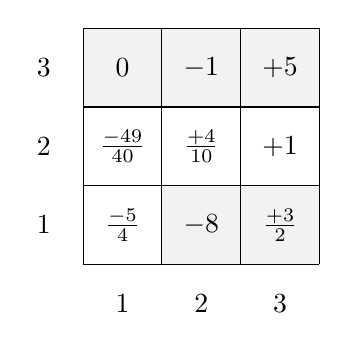
\begin{tikzpicture}
                \draw[step=1cm, black, thin] (0,0) grid (3,3);
                \fill[black, fill opacity=0.05] (1,0) rectangle (3,1);
                \fill[black, fill opacity=0.05] (0,2) rectangle (3,3);

                \draw (0.5, -0.5) node {1};
                \draw (1.5, -0.5) node {2};
                \draw (2.5, -0.5) node {3};
                \draw (-0.5, 0.5) node {1};
                \draw (-0.5, 1.5) node {2};
                \draw (-0.5, 2.5) node {3};

                \draw (0.5, 0.5) node {$\frac{-5}{4}$};
                \draw (1.5, 0.5) node {$-8$};
                \draw (2.5, 0.5) node {$\frac{+3}{2}$};
                \draw (0.5, 1.5) node {$\frac{-49}{40}$};
                \draw (1.5, 1.5) node {$\frac{+4}{10}$};
                \draw (2.5, 1.5) node {$+1$};
                \draw (0.5, 2.5) node {0};
                \draw (1.5, 2.5) node {$-1$};
                \draw (2.5, 2.5) node {$+5$};
            \end{tikzpicture}
        \end{figure}
    \end{solution}
\end{enumerate}

\newpage

\section{Q-learning}

An agent is in an unknown environment where there are three states $\cbk{A, B, C}$ and two actions $\cbk{0, 1}$. We are given the following tuples $(s, a, r, s')$, generated by taking actions in the environment.

\begin{table}[h]
    \centering
    \begin{tabular}{cccc}
        \toprule
        $s$ & $a$ & $r$ & $s'$ \\
        \midrule
        $A$ & $0$ & $+2$ & $A$ \\
        $C$ & $1$ & $-2$ & $A$ \\
        $B$ & $1$ & $+1$ & $B$ \\
        $A$ & $0$ & $-1$ & $B$ \\
        $B$ & $1$ & $-2$ & $C$ \\
        $C$ & $0$ & $+4$ & $B$ \\
        $B$ & $0$ & $+1$ & $A$ \\
        \bottomrule
    \end{tabular}
\end{table}

Assuming a discount factor $\gamma = 0.5$ and a learning rate $\alpha = 0.75$,

\begin{enumerate}
    \item Apply the $Q$-learning algorithm to obtain state-action-value $Q(s, a)$ estimates. Estimates are initialized to $0$.

    \begin{solution}
        As seen in the previous exercise, given trial trajectories of some policy $\pi$, it is possible to estimate its expected utility $V^\pi$ even without knowing the transition model $P(s' | s, a)$ or the reward function $R(s)$ of the environment. However, estimating $V^\pi$ only evaluates the quality of $\pi$, but does not describe how to improve it.

        By definition, the optimal policy $\pi^*$ is the one that maximizes the expect utility of the state $s$, \ie{}
        \begin{equation*}
            \pi^*(s) = \arg \max_a \sum_{s'} P(s' | s, a) V(s')
        \end{equation*}
        where $V(s) = \max_\pi V^\pi(s)$ is the state-value of $s$. Unfortunately, even if we knew $V$, we could not find the optimal actions without knowing the transition model. However, if we knew the state-action-value $Q(s, a)$ of taking action $a$ in state $s$, we would be able to select the optimal action
        \begin{equation*}
            \pi^*(s) = \arg \max_a Q(s, a) ,
        \end{equation*}
        where
        \begin{align*}
            Q(s, a) & = R(s) + \gamma \sum_{s'} P(s' | s, a) V(s') \\
            & = R(s) + \gamma \sum_{s'} P(s' | s, a) \max_{a'} Q(s', a')
        \end{align*}
        since $V(s) = \max_a Q(s, a)$. Fortunately, state-action-values $Q(s, a)$ can be learned in a model-free fashion using the $Q$-learning algorithm. Similarly to temporal-difference learning, in $Q$-learning, we perform stochastic gradient descent updates
        \begin{align*}
            \hat{Q}(s, a) & \gets \hat{Q}(s, a) - \alpha \rbk*{\hat{Q}(s, a) - r - \gamma \max_{a'} \hat{Q}(s', a')} \\
            & \gets (1 - \alpha) \hat{Q}(s, a) + \alpha \rbk*{r + \gamma \max_{a'} \hat{Q}(s', a')}
        \end{align*}
        from observed tuples $(s, r, a, s')$.

        In our case, the sequence of updates would be
        \begin{align*}
            \hat{Q}(A, 0) & \gets (1 - \alpha) \hat{Q}(A, 0) + \alpha \rbk*{2 + \gamma \max \cbk{\hat{Q}(A, 0), \hat{Q}(A, 1)}} = \frac{1}{4} 0 + \frac{3}{4} \rbk{2 + \frac{1}{2} 0} = \frac{+3}{2} \\
            \hat{Q}(C, 1) & \gets (1 - \alpha) \hat{Q}(C, 1) + \alpha \rbk*{-2 + \gamma \max \cbk{\hat{Q}(A, 0), \hat{Q}(A, 1)}} = \frac{1}{4} 0 + \frac{3}{4} \rbk{-2 + \frac{1}{2} \frac{3}{2}} = \frac{-15}{16} \\
            \hat{Q}(B, 1) & \gets (1 - \alpha) \hat{Q}(B, 1) + \alpha \rbk*{2 + \gamma \max \cbk{\hat{Q}(B, 0), \hat{Q}(B, 1)}} = \frac{1}{4} 0 + \frac{3}{4} \rbk{1 + \frac{1}{2} 0} = \frac{+3}{4} \\
            \hat{Q}(A, 0) & \gets (1 - \alpha) \hat{Q}(A, 0) + \alpha \rbk*{-1 + \gamma \max \cbk{\hat{Q}(B, 0), \hat{Q}(B, 1)}} = \frac{1}{4} \frac{3}{2} + \frac{3}{4} \rbk{-1 + \frac{1}{2} \frac{3}{4}} = \frac{-3}{32} \\
            \hat{Q}(B, 1)  & \gets \dots
        \end{align*}
        It should be noted that, as for TD learning, we are not limited to perform only one update for each tuple. Reusing tuples several times (in other orders) is a good way to reach convergence faster while generating less trials.
    \end{solution}

    \item We now switch to a feature-based estimator $\hat{Q}(s, a) = w_0 + w_1 f_1(s, a)$, with $f_1(s, a) = 2 a - 1$. Starting from weights $w_0 = w_1 = 0$, update the weights according to the approximate $Q$-learning algorithm.

    \begin{solution}
        We would like our estimates $\hat{Q}(s, a)$ to satisfy the
        Bellman equation, \ie{} to minimize
        \begin{equation*}
            L = \underset{s' | s, a}{\E} \sbk*{\rbk*{R(s) + \gamma \max_{a'} \hat{Q}(s', a') - \hat{Q}(s, a)}^2} .
        \end{equation*}
        To reach this objective we follow the opposite of its gradient
        \begin{equation*}
            \nabla_{\!w} L = 2 \underset{s' | s, a}{\E} \sbk*{\rbk*{\hat{Q}(s, a) - R(s) - \gamma \max_{a'} \hat{Q}(s', a')} \nabla_{\!w} \hat{Q}(s, a)}
        \end{equation*}
        with respect to the weights\footnotemark{} $w$ of $\hat{Q}(s, a)$. Once again, due to the expectation, we are forced to use a stochastic approximation of the gradient from observed tuples $(s, a, r, s')$ and to update the weights as
        \begin{equation*}
            w \gets w - \alpha \rbk*{\hat{Q}(s, a) - r - \gamma \max_{a'} \hat{Q}(s', a')} \nabla_w \hat{Q}(s, a) ,
        \end{equation*}
        where $\alpha$ is the learning rate. In our case,
        \begin{equation*}
            \nabla_{\!w} \hat{Q}(s, a) = \mat{\partial_{w_0} \\ \partial_{w_1} } (w_0 + w_1 f_1(s, a)) = \mat{ 1 \\ f_1(s, a)} = \mat{1 \\ 2 a - 1}
        \end{equation*}
        and the two first weight updates would be
        \begin{align*}
            w & \gets w - \alpha \rbk*{\hat{Q}(A, 0) - 2 - \gamma \max \cbk{\hat{Q}(A, 0), \hat{Q}(A, 1)}} \nabla_{\!w} \hat{Q}(A, 0) \\
            & \gets \mat{0 \\ 0} - \frac{3}{4} \rbk*{-2 - \frac{1}{2} \max\cbk{0, 0}} \mat{1 \\ -1} = \mat{\frac{+3}{2} \\ \frac{-3}{2}} \\
            w & \gets w - \alpha \rbk*{\hat{Q}(C, 1) + 2 - \gamma \max \cbk{\hat{Q}(A, 0), \hat{Q}(A, 1)}} \nabla_{\!w} \hat{Q}(C, 1) \\
            & \gets \mat{\frac{+3}{2} \\ \frac{-3}{2}} - \frac{3}{4} \rbk*{2 - \frac{1}{2} \max\cbk{0, 3}} \mat{1 \\ 1} = \mat{\frac{+9}{8} \\ \frac{-15}{8}} .
        \end{align*}

        \footnotetext{It should be noted that the target $R(s) + \gamma \max_{a'} \hat{Q}(s', a')$ should not affected by the gradient operation as it is considered constant in the objective. In practice, this is not true as modifying the weights in a parametric function $\hat{Q}$ does so for all state-action pairs $(s, a)$ at once. This generally makes the approximate $Q$-learning algorithm very unstable.}
    \end{solution}
\end{enumerate}

\newpage

\section{Football}

\def\C{\texttt{C}}
\def\A{\texttt{A}}
\def\F{\texttt{F}}
\def\G{\texttt{G}}
\def\P{\texttt{P}}
\def\S{\texttt{S}}

ULiège's football team is playing against UCL's team next week. With a lot of losses this season, Liège needs to improve their attack strategy to win the game and increase their popularity. Luckily, the team captain follows INFO8006 and knows how to model the attack as a Markov Decision Process. The captain considers four states \texttt{close} (\C), \texttt{away} (\A), \texttt{fail} (\F), and \texttt{goal} (\G), and two actions \texttt{pass} (\P) and \texttt{shoot} (\S). Although the transition probabilities are unsure, the possible transitions $(s, a, s')$ are known. To each transition is associated an increase/decrease of the team's popularity.

\begin{table}[h]
    \centering
    \begin{tabular}{ccc|c}
        \toprule
         $s$ & $a$ & $s'$ & $R(s, a, s')$ \\
         \midrule
         \C & \P & \C & $+1$ \\
         \C & \P & \A & $-1$ \\
         \C & \P & \F & $-2$ \\
         \C & \S & \C & $+3$ \\
         \C & \S & \F & $-5$ \\
         \C & \S & \G & $+10$ \\
         \midrule
         \A & \P & \C & $+2$ \\
         \A & \P & \A & $0$ \\
         \A & \P & \F & $-3$ \\
         \A & \S & \C & $+3$ \\
         \A & \S & \F & $-10$ \\
         \A & \S & \G & $+20$ \\
         \bottomrule
    \end{tabular}
\end{table}

The current strategy of the team is to always shoot. Last match, they had several attack opportunities, resulting in the following actions.

\begin{table}[h]
    \centering
    \begin{tabular}{c|cccccccc}
        \toprule
         $s$ & \C & \C & \C & \C & \A & \A & \A & \A \\
         $a$ & \S & \S & \S & \S & \S & \S & \S & \S \\
         $s'$ & \G & \C & \G & \F & \F & \C & \F & \F \\
         \bottomrule
    \end{tabular}
\end{table}

Assuming a discount factor $\gamma = 0.75$ and a learning rate $\alpha = 0.25$,

\begin{enumerate}
    \item Build an estimator of the transition model $P(s' | s, a)$ and, from it, determine the expected utility $V^\pi$ of the team's current policy $\pi$.
    \begin{solution}
        Given the previous table, we can estimate the transition probabilities for $s \in \cbk{\C, \A}$ and $a = \S$.

        \begin{table}[h]
            \centering
            \begin{tabular}{cc|cccc}
                \toprule
                 $s$ & $a$ & \multicolumn{4}{c}{$P(s' | s, a)$} \\
                     &     & \C & \A & \F & \G \\
                 \midrule
                 \C & \S & $0.25$ & $0$ & $0.25$ & $0.5$ \\
                 \A & \S & $0.25$ & $0$ & $0.75$ & $0$ \\
                 \bottomrule
            \end{tabular}
        \end{table}

        We can now determine the expected utility $V^\pi$ of the team's current policy $\pi(s) = \S$ using the following Bellman operator
        \begin{equation*}
            V_{i + 1}^\pi(s) = \sum_{s'} P(s' | s, \pi(s)) \sbk*{R(s, \pi(s), s') + \gamma V_i^\pi(s')} ,
        \end{equation*}
        with $V_0^\pi(s) = 0$ for all state $s$. Because the states \F and \G are terminal, their expected utility remains constant and we only have to update \C and \A. For the first iteration,
        \begin{align*}
            V_1^\pi(\C) & = \sum_{s'} P(s' | \C, \S) \sbk*{R(\C, \S, s') + \gamma V_0^\pi(s')} \\
            & = 0.25 (3 + \gamma \, 0) + 0.25 (-5 + \gamma \, 0) + 0.5 (10 + \gamma \, 0) = 4.5
        \end{align*}
        and
        \begin{align*}
            V_1^\pi(\A) & = \sum_{s'} P(s' | \A, \S) \sbk*{R(\A, \S, s') + \gamma V_0^\pi(s')} \\
            & = 0.25 (3 + \gamma \, 0) + 0.75 (-10 + \gamma \, 0) = -6.75 .
        \end{align*}
        We repeat the same procedure until $V_{i + 1}^\pi(s) \approx V_i^\pi(s)$ for all state $s$.

        \begin{table}[h]
            \centering
            \begin{tabular}{c|cccc}
                \toprule
                $s$ & \C & \A & \F & \G \\
                \midrule
                $V_0^\pi(s)$ & 0 & 0 & 0 & 0 \\
                $V_1^\pi(s)$ & 4.5 & -6.75 & 0 & 0 \\
                $V_2^\pi(s)$ & \num{5.3437} & \num{-5.9063} & 0 & 0 \\
                $V_3^\pi(s)$ & \num{5.5019} & \num{-5.7480} & 0 & 0 \\
                $V_4^\pi(s)$ & \num{5.5316} & \num{-5.7183} & 0 & 0 \\
                \vdots       & \vdots & \vdots & \vdots & \vdots \\
                $V_8^\pi(s)$ & \num{5.5385} & \num{-5.7115} & 0 & 0 \\
                \bottomrule
            \end{tabular}
        \end{table}
    \end{solution}

\end{enumerate}

The captain found the tapes of the previous season where they had much more success. Together with the team, the captain selects the following instructive actions.

\begin{table}[h]
    \centering
    \begin{tabular}{c|cccccccc}
        \toprule
         $s$ & \C & \C & \A & \A & \C & \A & \A & \C \\
         $a$ & \S & \S & \S & \P & \P & \P & \S & \P \\
         $s'$ & \G & \C & \F & \C & \C & \C & \F & \F \\
         \bottomrule
    \end{tabular}
\end{table}

\begin{enumerate}
    \setcounter{enumi}{1}
    \item Given the selected tuples, apply the $Q$-learning algorithm to obtain state-action-value $Q(s, a)$ estimates. Estimates are initialized to 0.

    \begin{solution}
        In $Q$-learning, the state-action-value $Q(s, a)$ estimates are updated following
        \begin{align*}
            Q(s, a) & \gets Q(s, a) - \alpha \rbk*{Q(s, a) - r - \gamma \max_{a'} Q(s', a')} \\
            & \gets (1 - \alpha) Q(s, a) + \alpha \rbk*{r + \gamma \max_{a'} Q(s', a')}
        \end{align*}
        for observed tuples $(s, r, a, s')$. In our case, we have a list a 16 (8 + 8) tuples $(s, a, s')$ and we have access to the reward function $R(s, a, s')$. Using the tuples in arbitrary order, we have
        \begin{align*}
            Q(\C, \S) & \gets (1 - \alpha) Q(\C, \S) + \alpha \rbk*{R(\C, \S, \G) + \gamma \max_{a'} Q(\G, a')} \\
            & \gets 0.75 \times 0 + 0.25 \rbk{10 + 0} = 2.5 \\
            Q(\C, \S) & \gets (1 - \alpha) Q(\C, \S) + \alpha \rbk*{R(\C, \S, \C) + \gamma \max_{a'} Q(\C, a')} \\
            & \gets 0.75 \times 2.5 + 0.25 \rbk{3 + 0.75 \max \cbk{2.5, 0}} = 3.094 \\
            Q(\A, \S) & \gets (1 - \alpha) Q(\A, \S) + \alpha \rbk*{R(\A, \S, \F) + \gamma \max_{a'} Q(\F, a')} \\
            & \gets 0.75 \times 0 + 0.25 \rbk{-10 + 0} = -2.5 \\
            Q(\A, \P) & \gets (1 - \alpha) Q(\A, \P) + \alpha \rbk*{R(\A, \P, \C) + \gamma \max_{a'} Q(\C, a')} \\
            & \gets 0.75 \times 0 + 0.25 \rbk{2 + 0.75 \max \cbk{3.094, 0}} = 4.320 \\
            Q(\C, \P) & \gets \dots
        \end{align*}
    \end{solution}

    \item Determine the optimal policy according to the state-action-value estimates.

    \begin{solution}
        \begin{equation*}
            \pi(s) = \begin{cases}
                \S & \text{if } s = \C \\
                \P & \text{if } s = \A
            \end{cases}
        \end{equation*}
    \end{solution}
\end{enumerate}

\newpage

\section*{Supplementary materials}

\begin{itemize}
    \item Playing Atari with Deep Reinforcement Learning

    \qrcode{https://arxiv.org/abs/1312.5602}

    \item Chapter 21 of the reference textbook.
\end{itemize}

\end{document}
